%
% fig-morse.tex
%
% (c) 2025 Prof Dr Andreas Müller
%
\begin{figure}
\centering
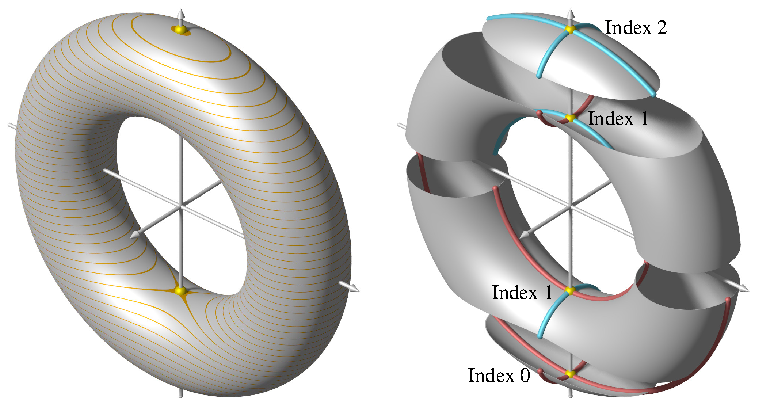
\includegraphics{chapters/120-topologie/images/morse.pdf}
\caption{Links: Torus mit Höhenlinien der Funktion $f(p) = z(p)$ für Punkte
$p$ auf dem Torus.
\index{Torus}%
Kritische Punkte von $f$ sind gelb eingezeichnet.
\index{kritischer Punkt}%
Rechts: Der Torus lässt sich in Teile zerlegen, die jeweils genau
einen kritischen Punkte enthalten. Aus den Indizes der kritischen Punkte
\index{Index}%
lassen sich topologische Eigenschaften der Mannigfaltigkeit rekonstruieren.
\label{buch:topologie:fig:morse}}
\end{figure}
